\chapter{Experiment 1 - AnnotateMe}
\label{appendix1:annotatme}

\section{Documentation of RabbitMQ Message Routes}
\label{appendix1:AMQPDOCsec}
The table below represents all the communication infrastructure for the asynchronous publish-subscribe messages protocol. All microservices composing the NED Framework exchange information with each other by publishing and subscribing to each-others' message queues using RabbitMQ as the underlying technology provider. All the parameters associated with each communication route (Routing Key - Column 1), are mandatory and shall be provided as a complete JSON object with the specified name and the corresponding data type.
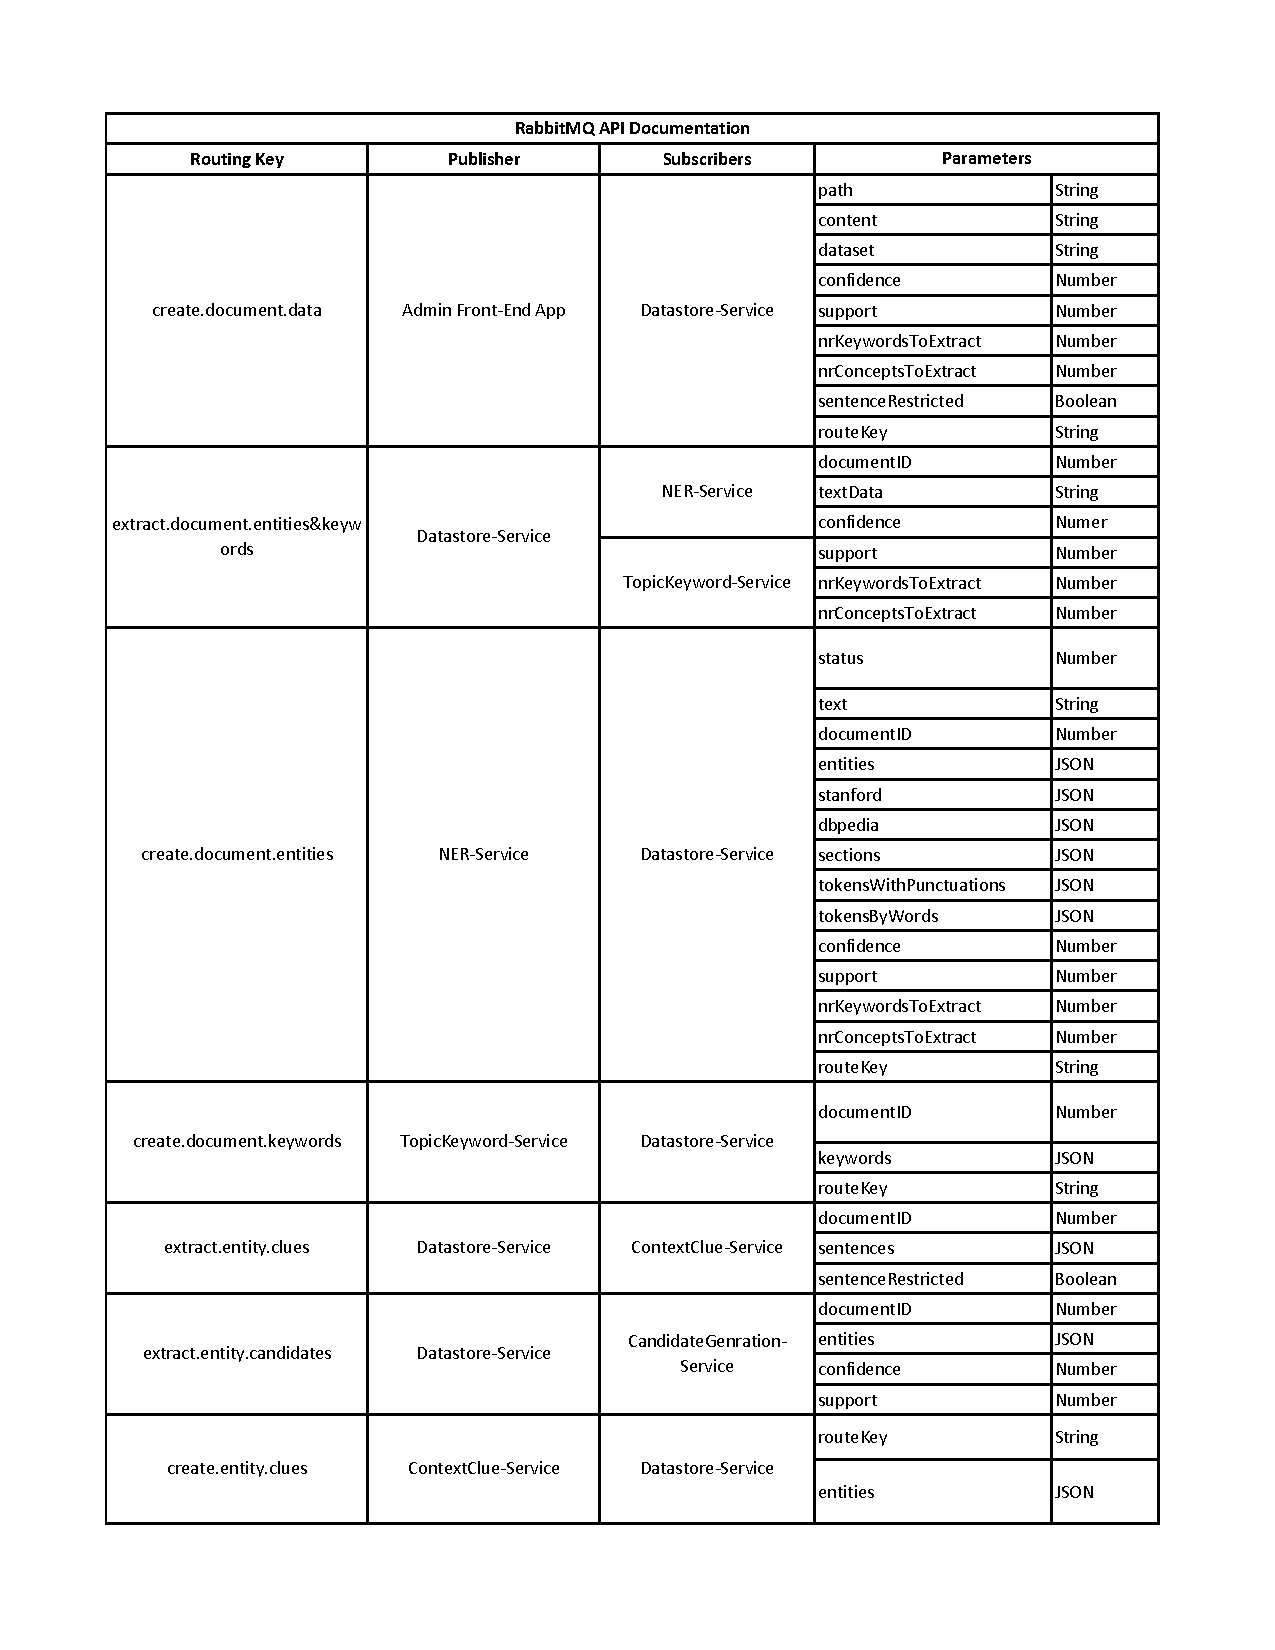
\includepdf[scale=0.7,pages=-]{appendices/rabbitmq-doc.pdf}

\section{Documentation of Datastore and Dataprep Microservice REST routes}
\label{appendix1:RESTDOCsec}
This appendix documents all the routes used to access the resources residing in the \textbf{Datastore Microservice} as well as the documented routes for accessing resources from the \textbf{Dataprep Microservice}. Swagger Documentation API\footnote{Swagger IO \url{http://swagger.io/}} has been used for generating the documentation schema illustrated below.

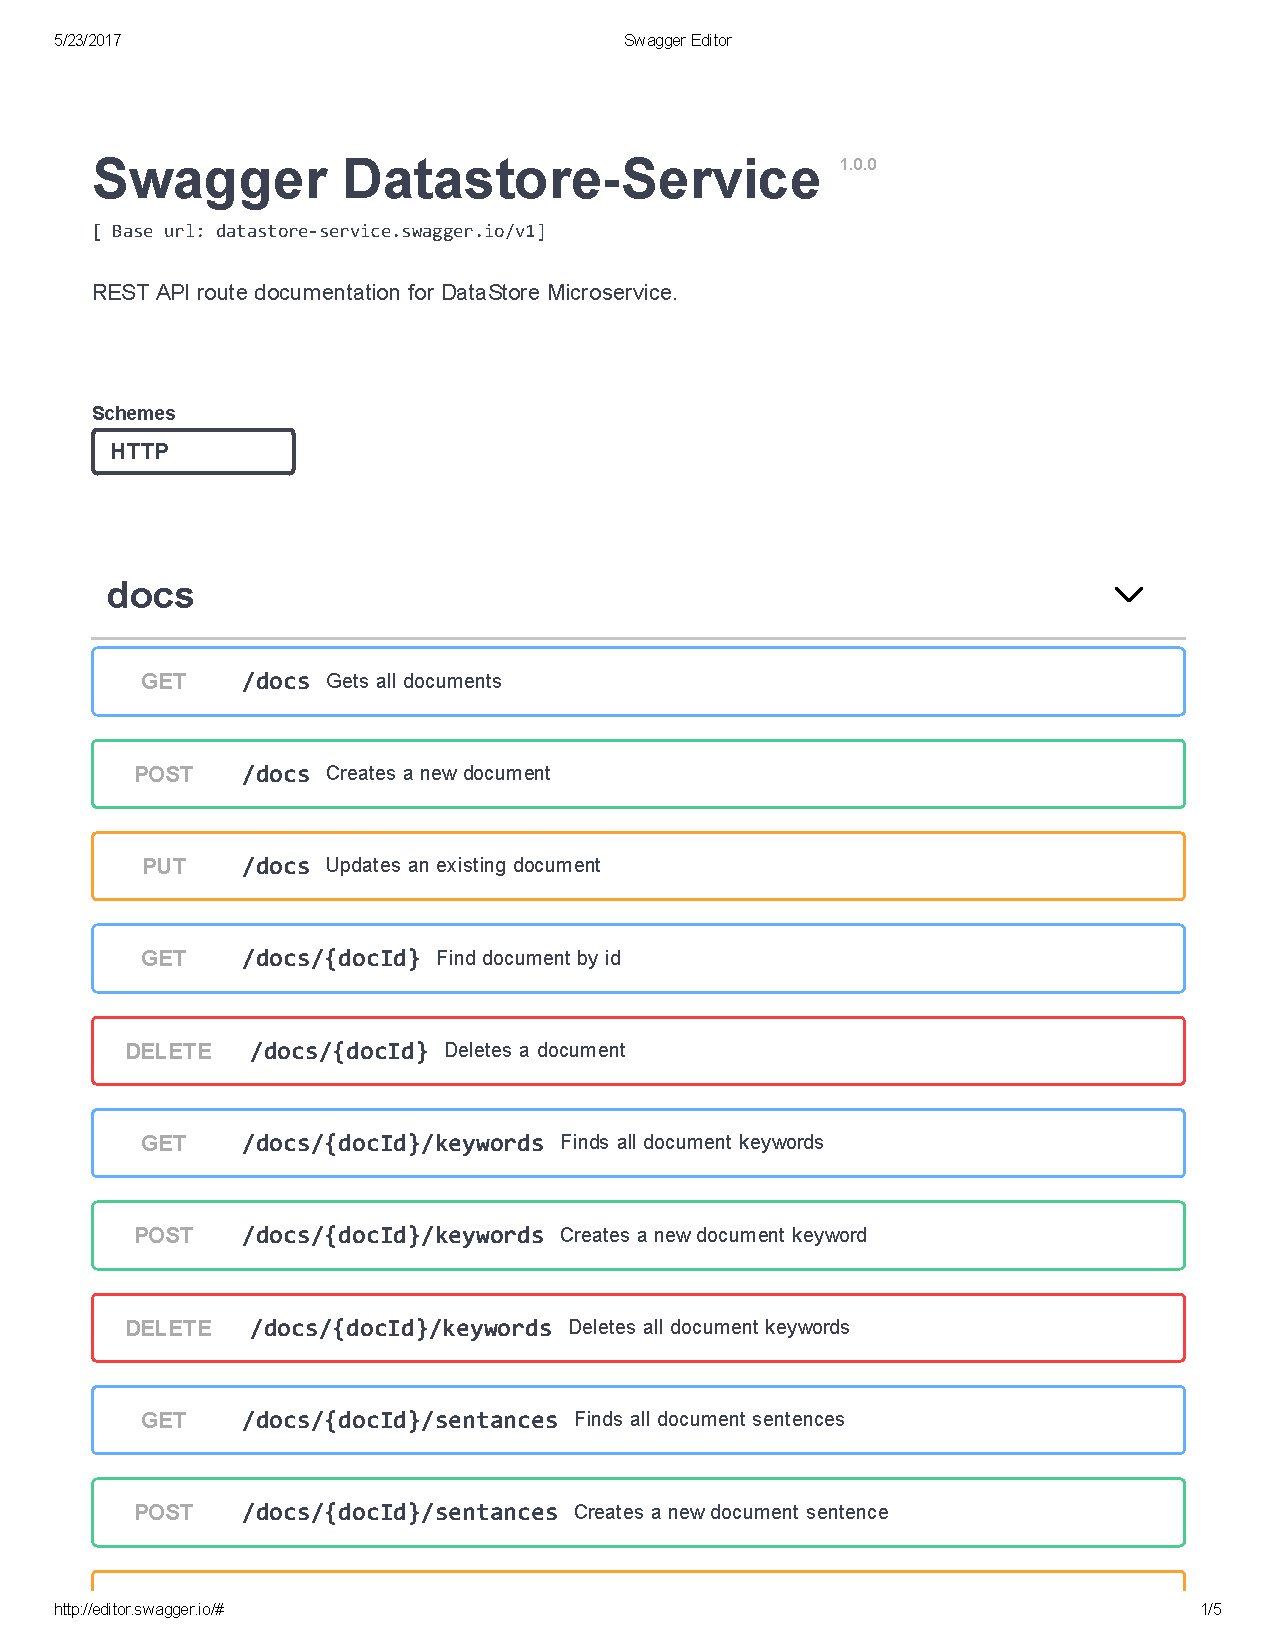
\includepdf[scale=0.7,pages=-]{appendices/swagger-datastore-service-documentations.pdf}
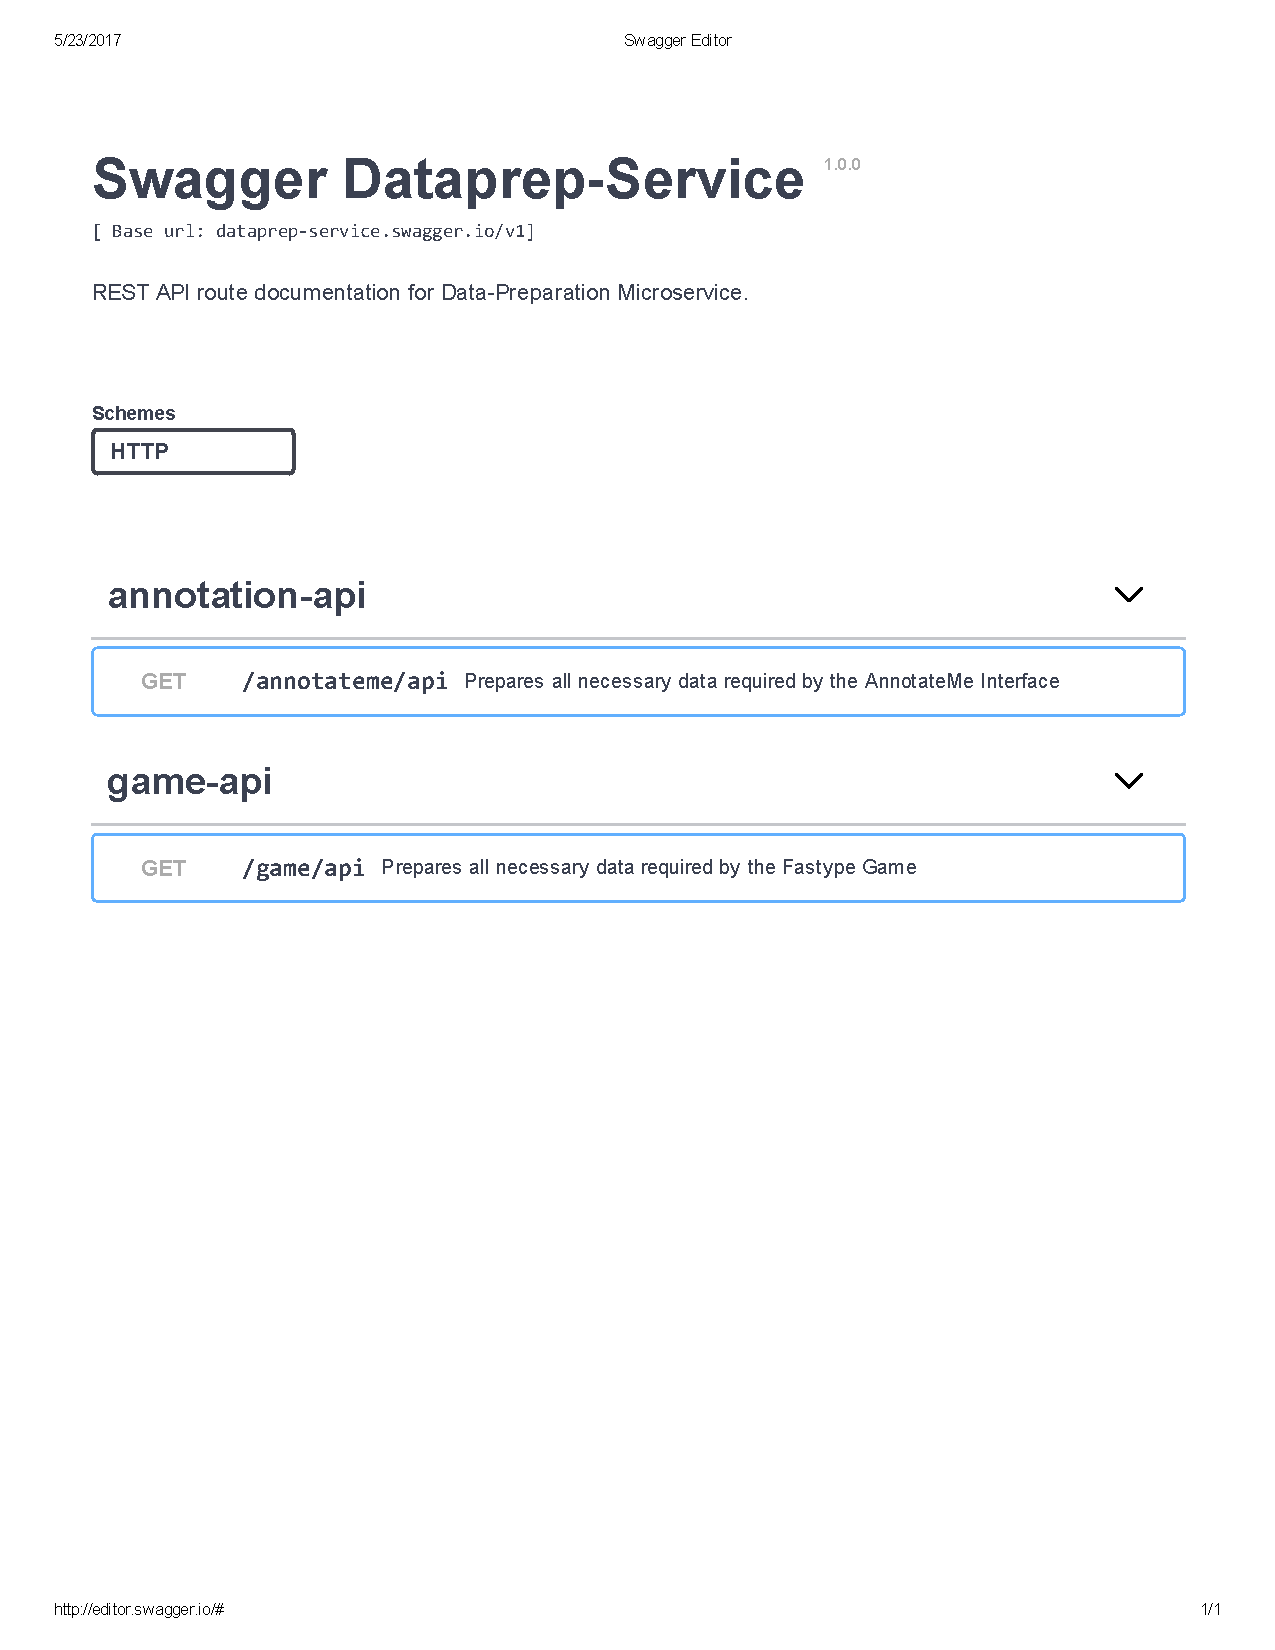
\includepdf[scale=0.7,pages=-]{appendices/swagger-dataprep-service-documentations.pdf}


%Ex1 - Consent Form
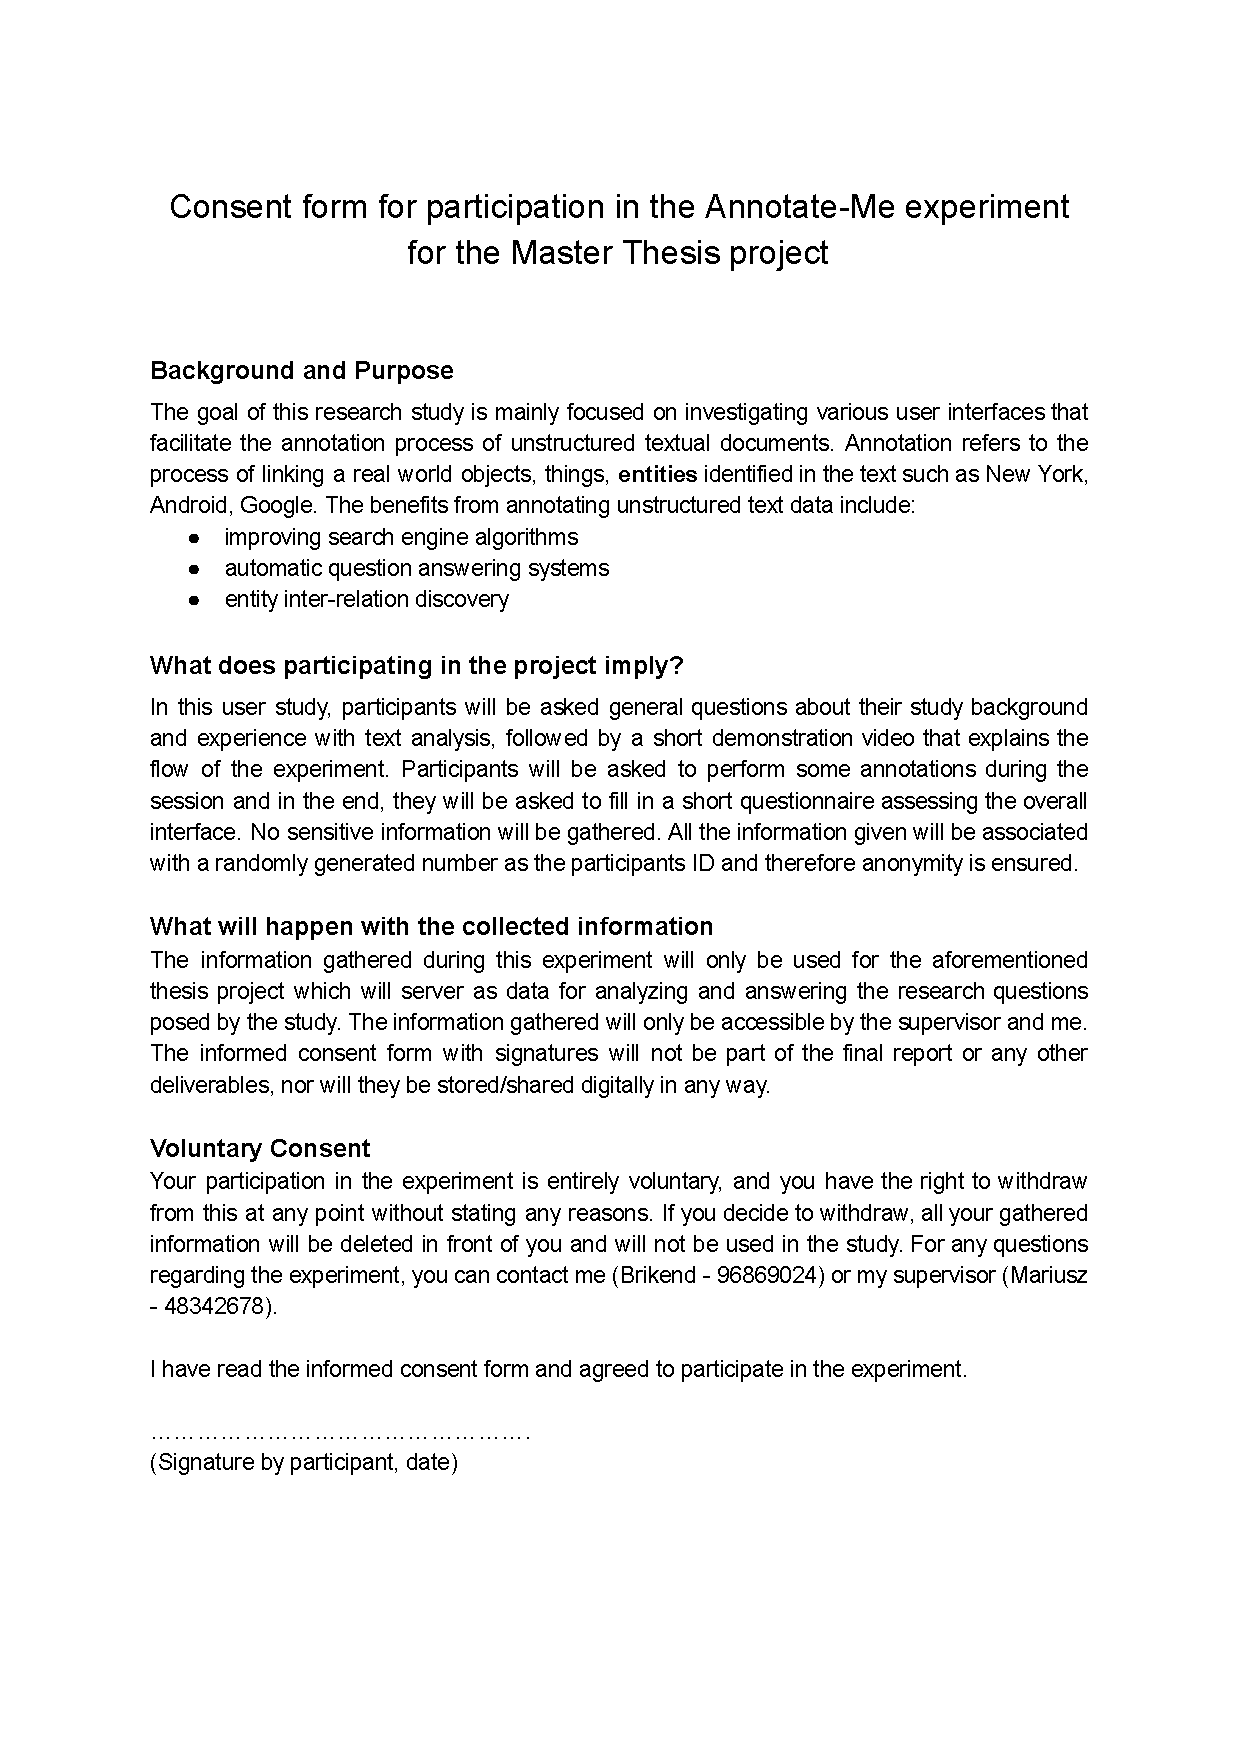
\includepdf[scale=0.8,pages=1,pagecommand=\section{Consent Form}]{appendices/experiment1-consentform.pdf}

%Ex1 - Pre Questionnaire
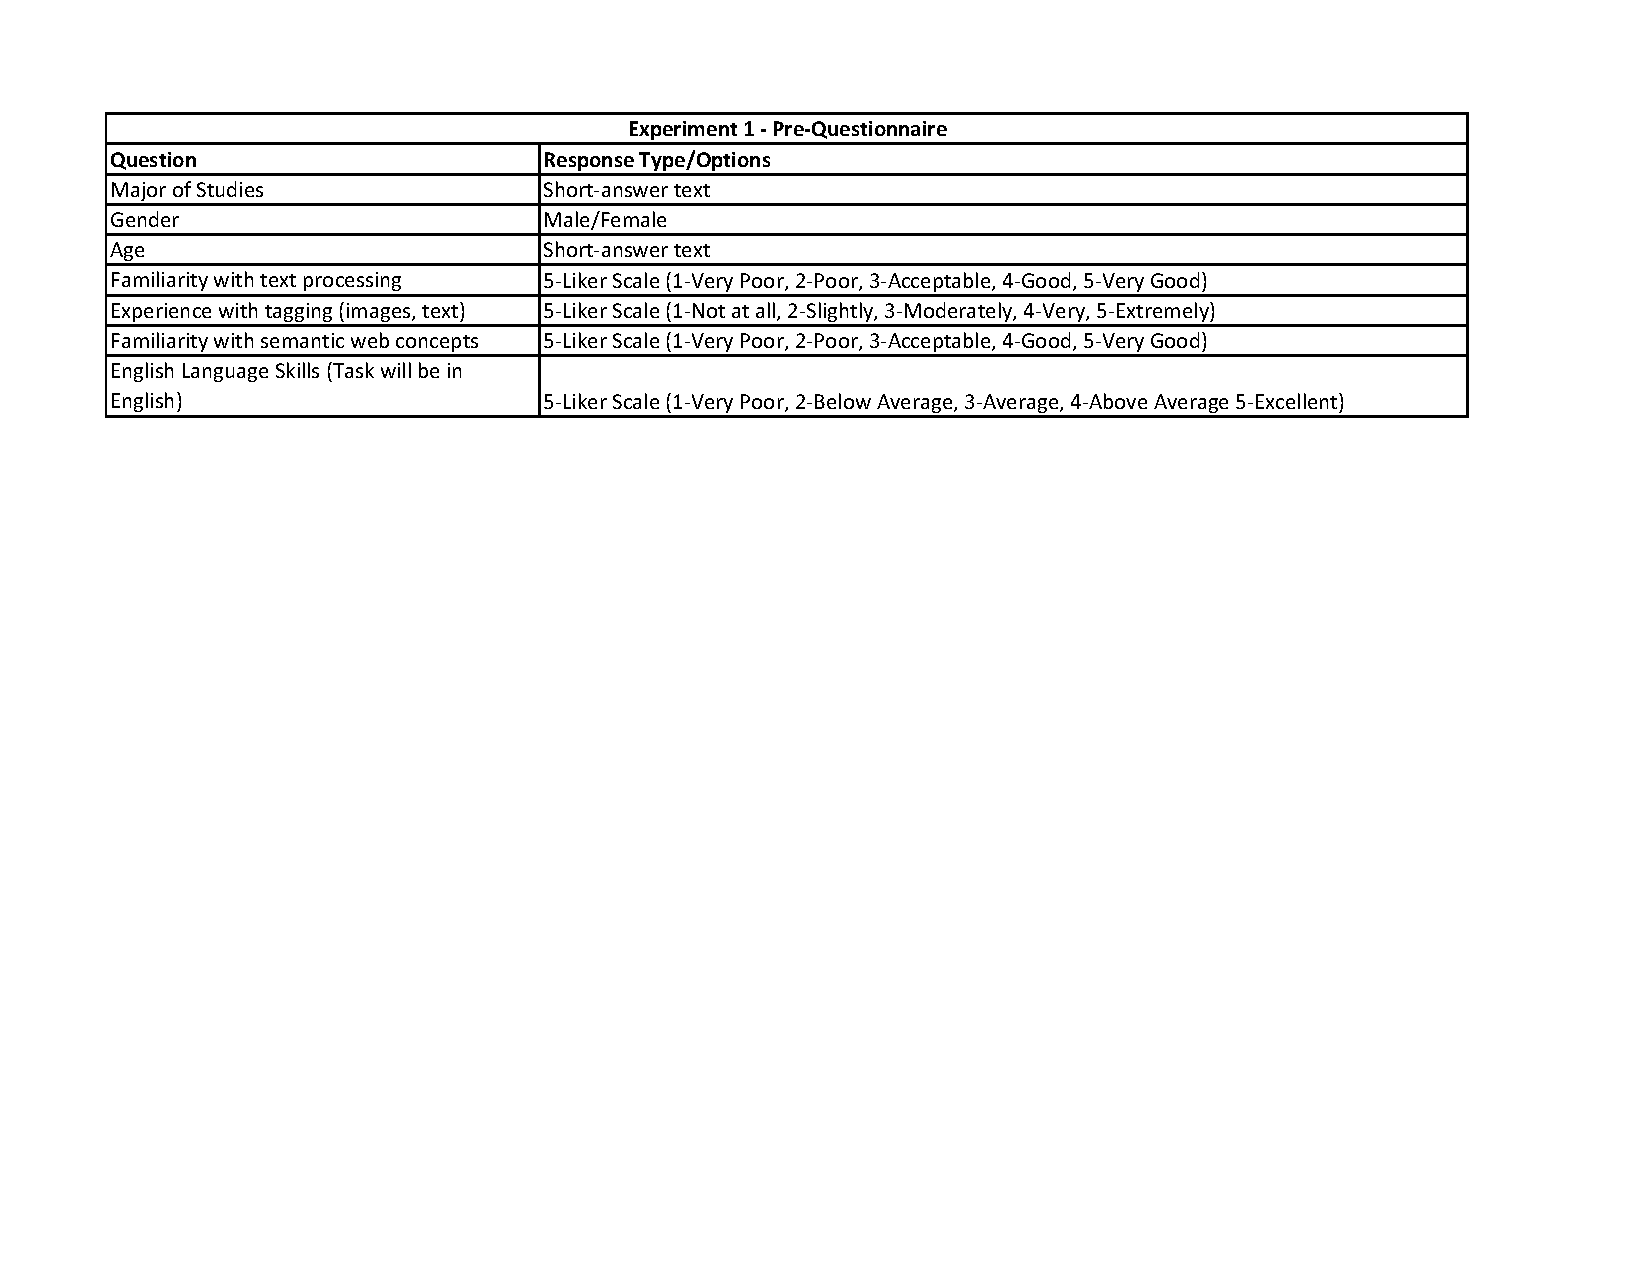
\includepdf[scale=0.8,angle=90,pagecommand=\section{Pre-Questionnaire }]{appendices/pre-questionnaire.pdf}

%Ex2 - Post Questionnaire
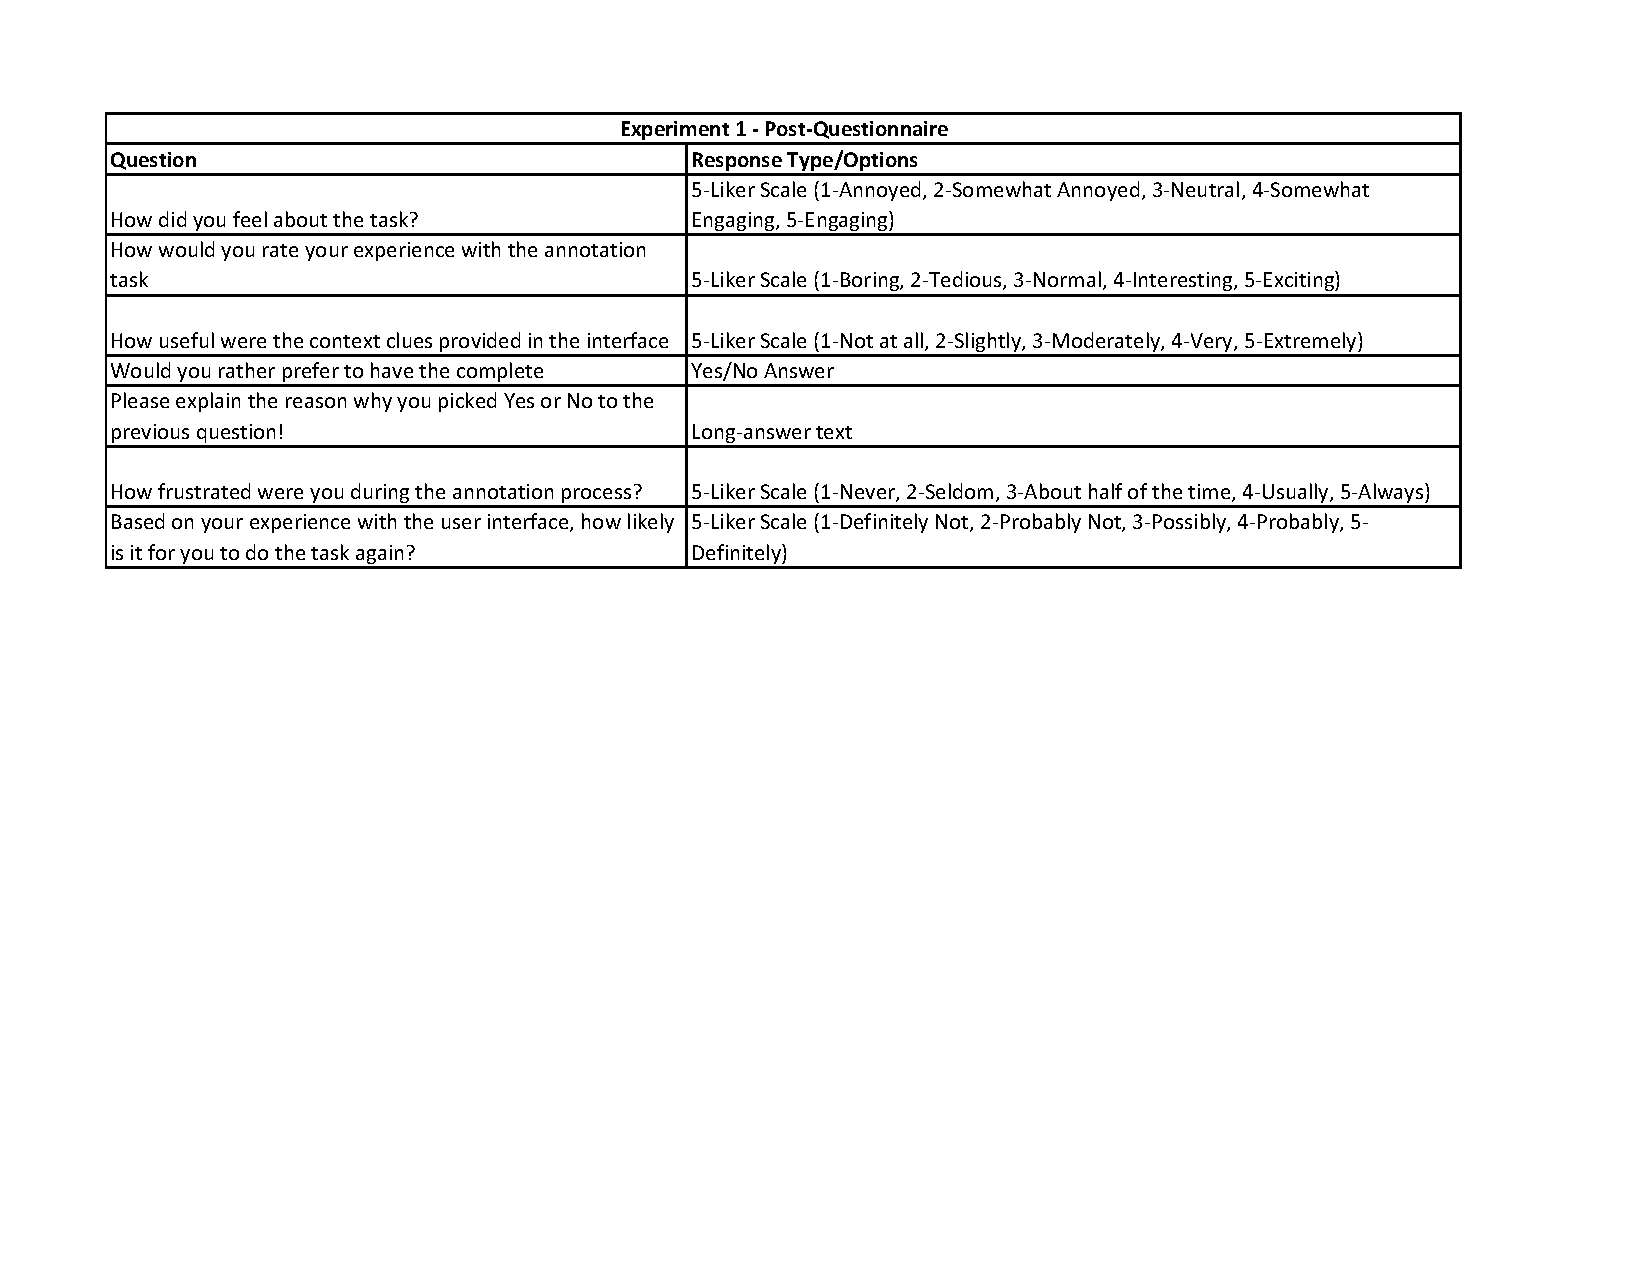
\includepdf[scale=0.8,angle=90,pagecommand=\section{Post-Qestionnaire }]{appendices/ex1-postquestionnaire.pdf}

\chapter{Experiment 2 - Fastype}
\label{appendix2:fastype}

%Ex2 - Consent Form
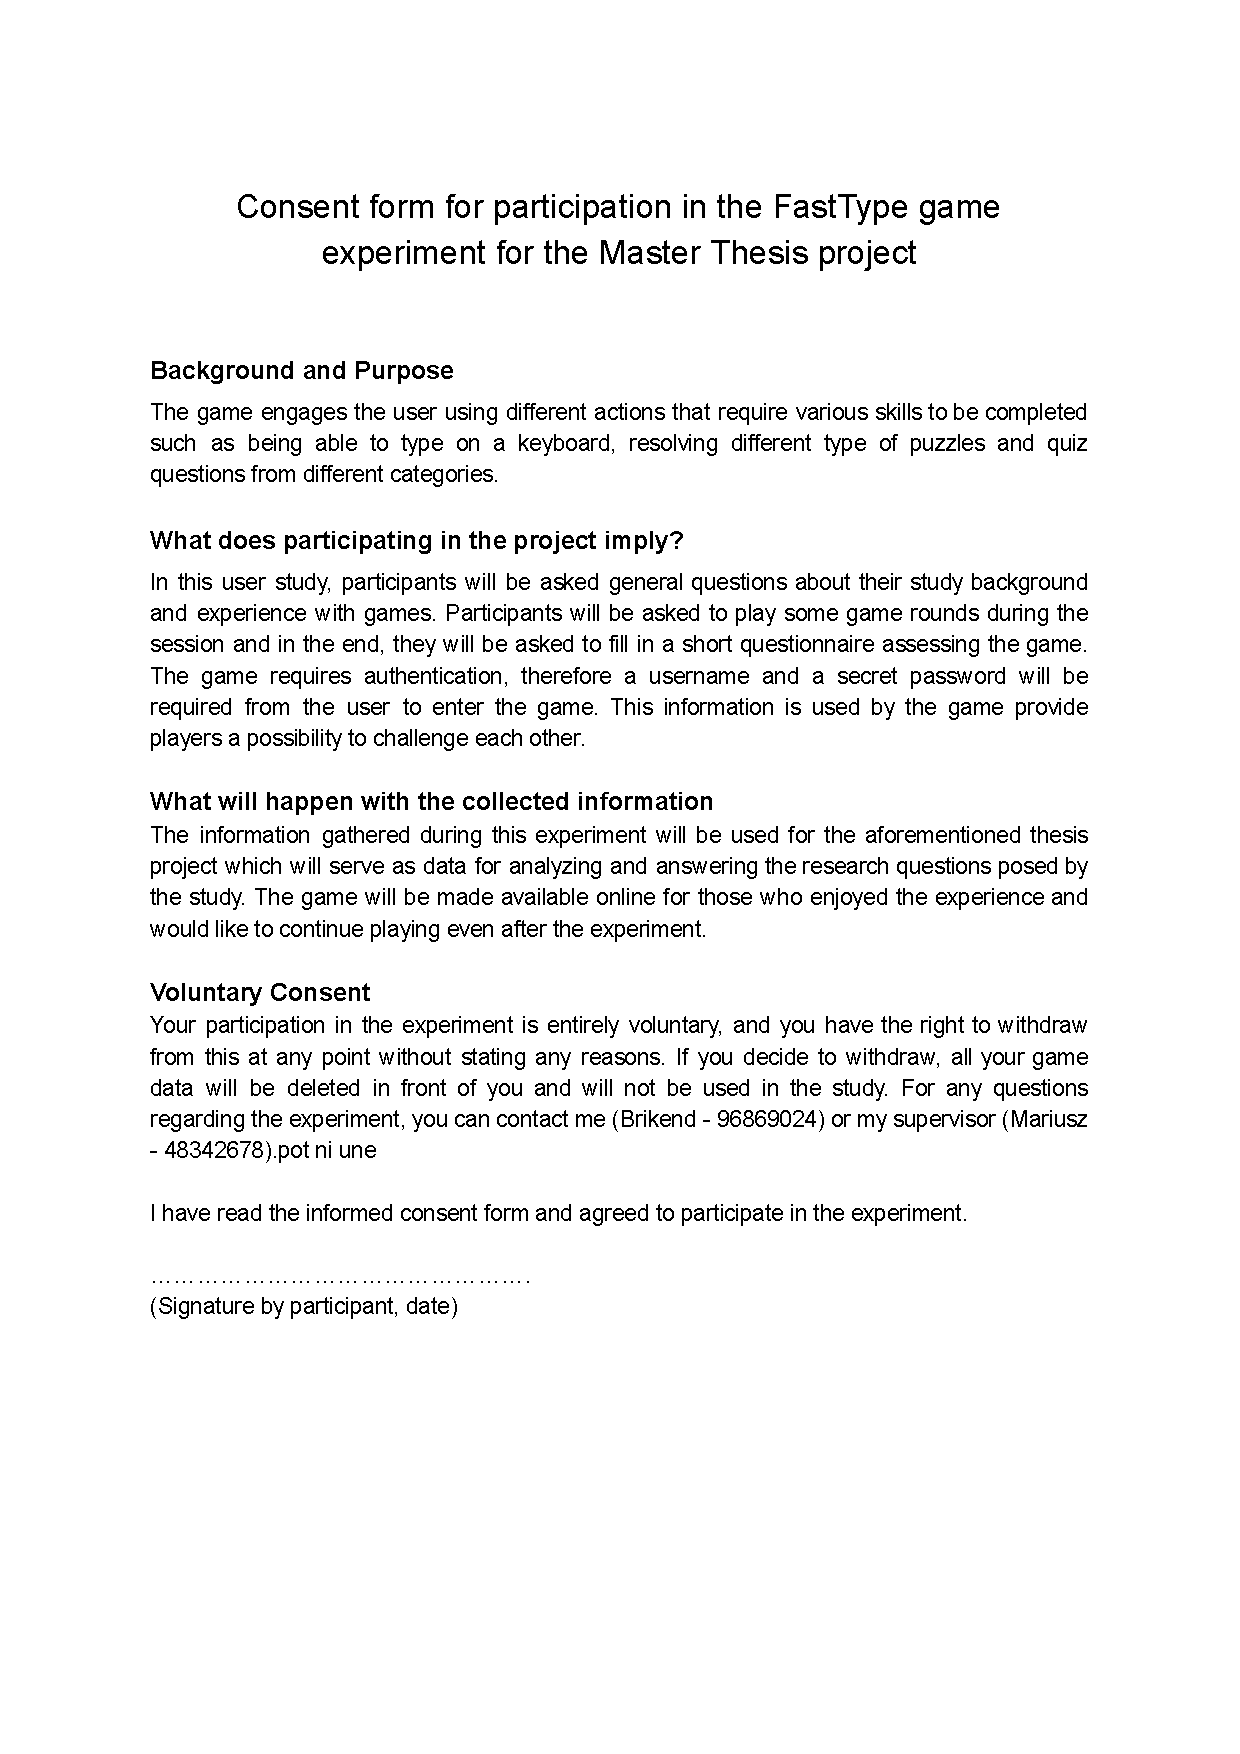
\includepdf[scale=0.8,pages=1,pagecommand=\section{Consent Form}]{appendices/ex2-consentform.pdf}

%Ex1 - Pre Questionnaire
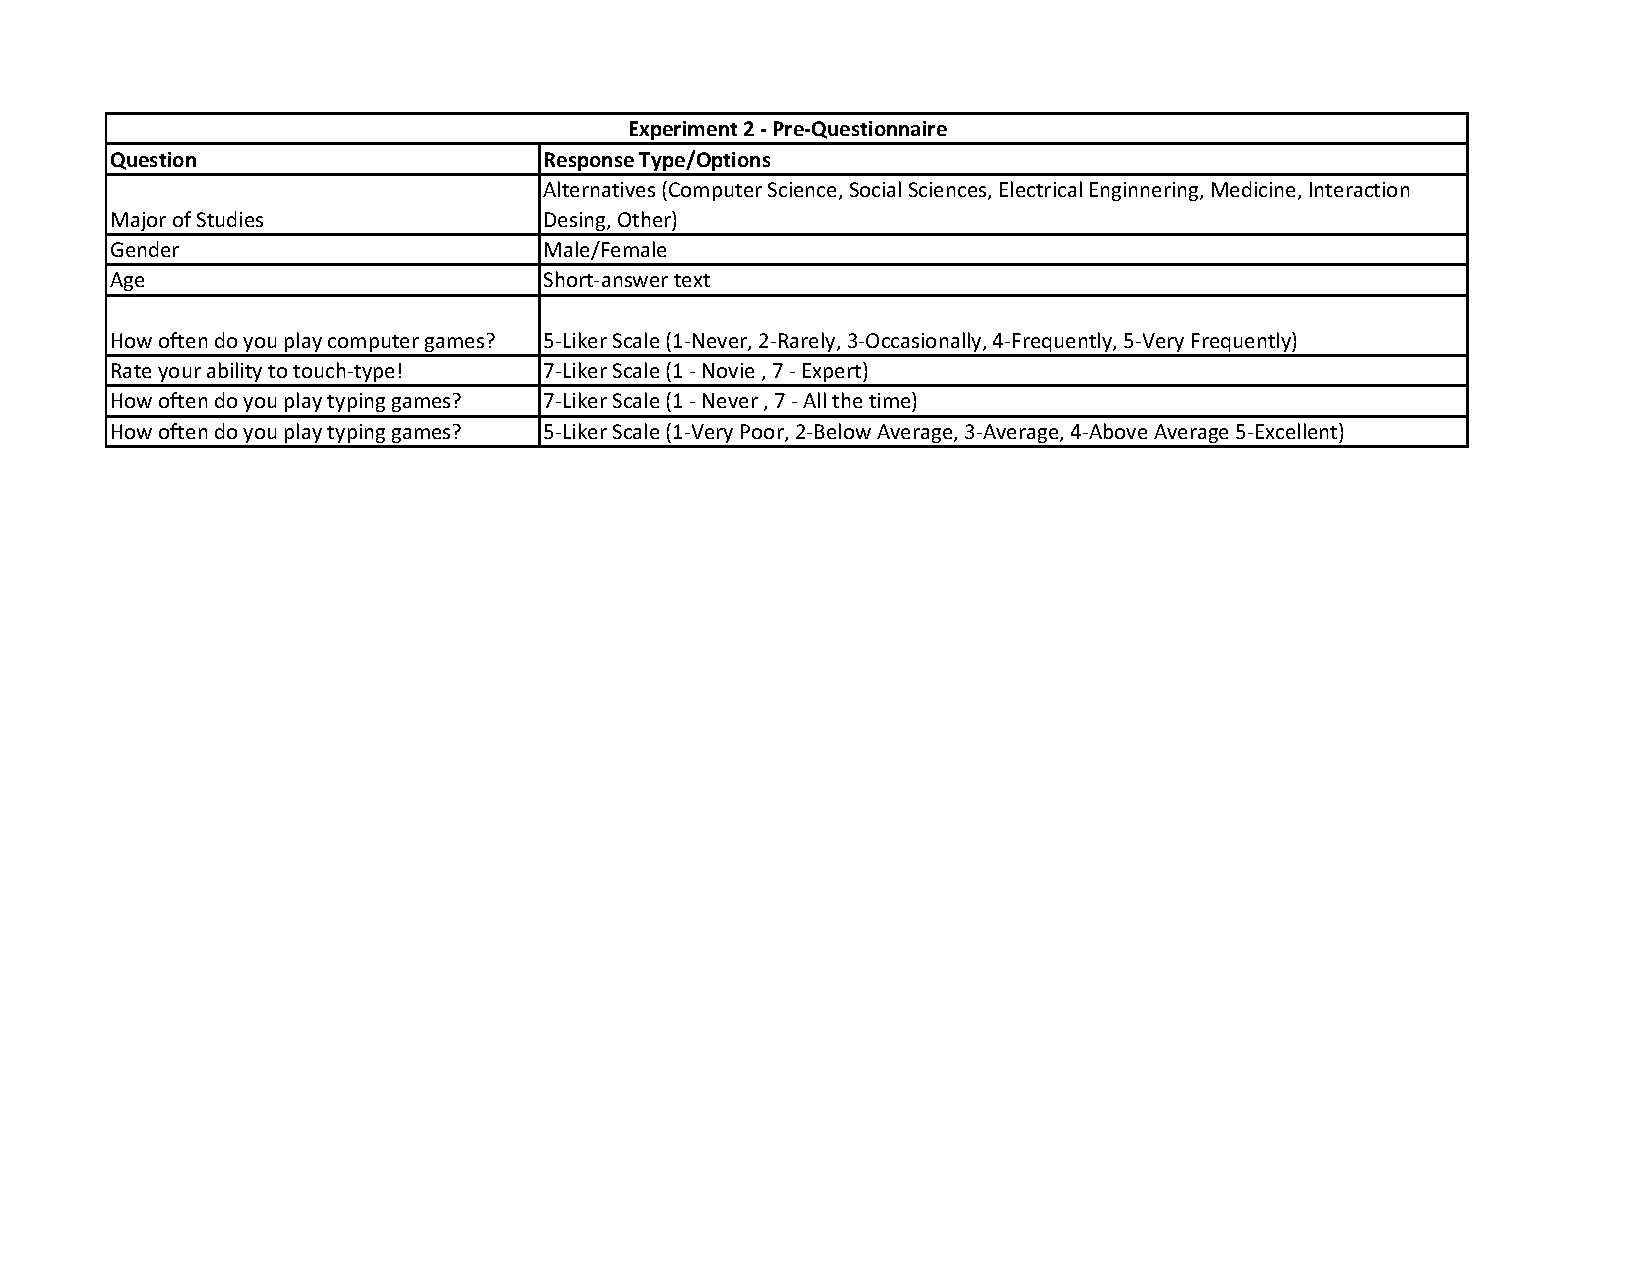
\includepdf[scale=0.8,angle=90,pagecommand=\section{Pre-Questionnaire }]{appendices/ex2-prequestionnaire.pdf}

%Ex2 - Post Questionnaire
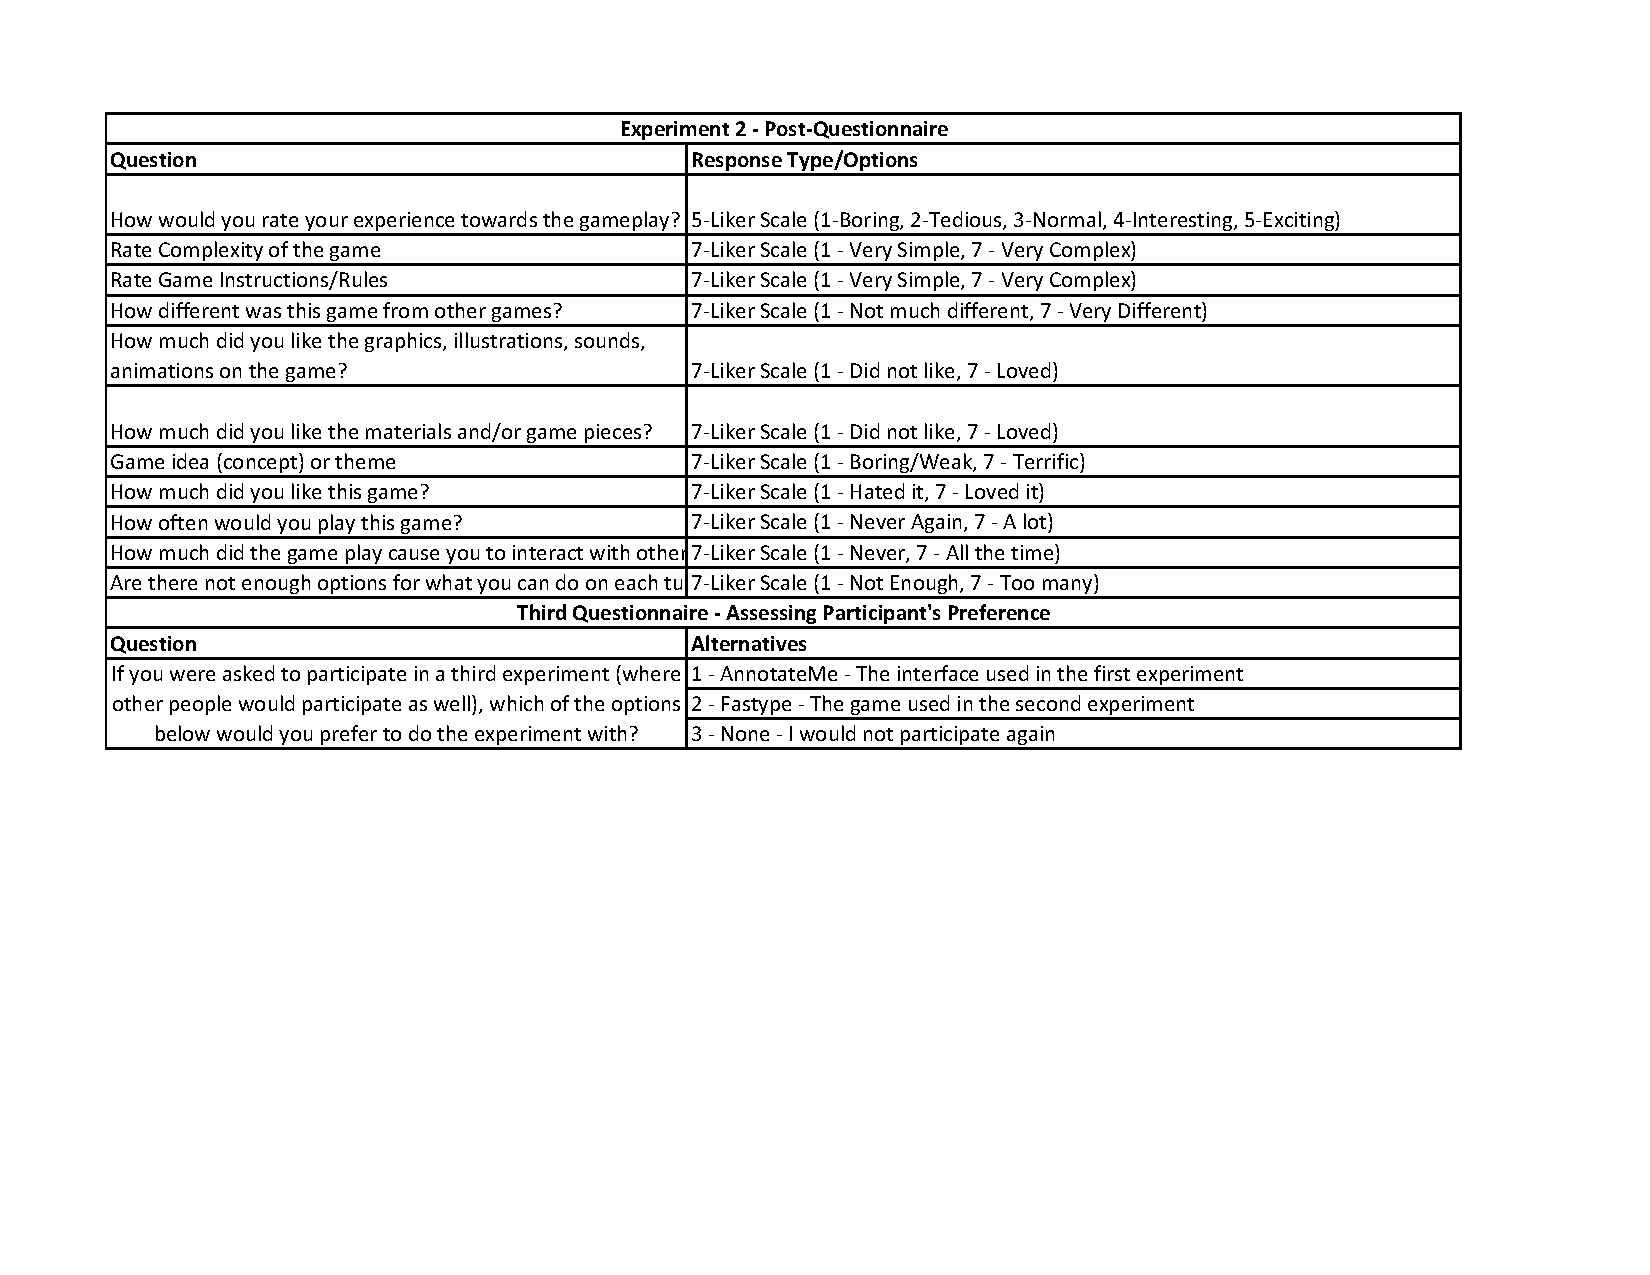
\includepdf[scale=0.8,angle=90,pagecommand=\section{Post-Questionnaire \& Preference Questionnaire }]{appendices/ex2-post-both.pdf}

\chapter{Anova - Raw Data Analysis}
\label{appendix3:chapter}


\section{Attractiveness of Interfaces}
\label{appendix3:attractiveness_analysis}
Below we present the Anova calculations performed on the gathered observations when asked participants about their experience with both interfaces. 

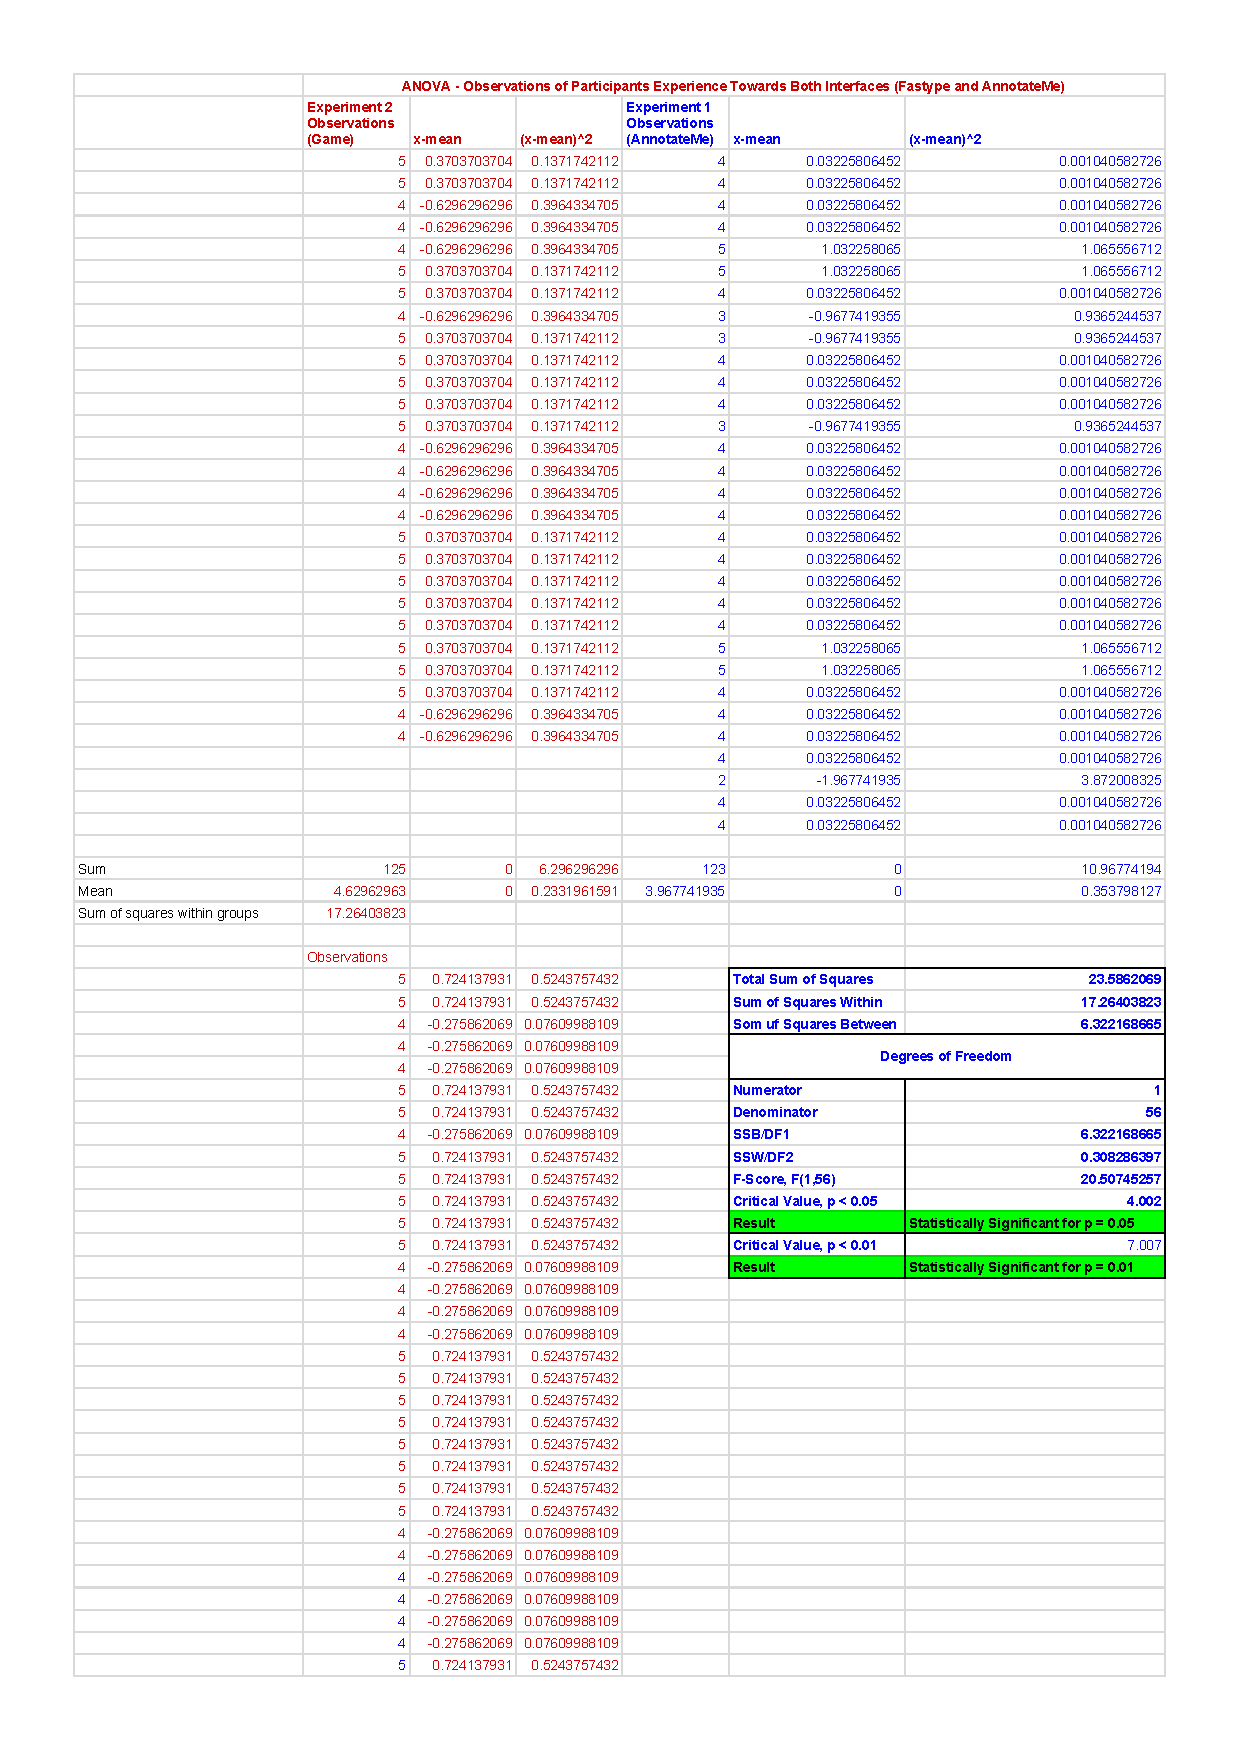
\includepdf[scale=0.7,pages=-]{appendices/anova-participant-experince.pdf}

\section{Player Engagement Analysis}
\label{appendix3:engagement_analysis}
The analysis presented below represent the Anova analysis performed on the gathered observations when participants where asked to rate their engagement with both interfaces using a liker-scale measure\footnote{For the first experiment we used 5-liker scale whereas for the second experiment we used a 7-liker scale. We normalize the observations afterwards to accurately perform comparison measures}. Please note that different measure metrices were used in each experiment, however, a normalization procedure is performed for the game observation to scale the values down from a 7-liker scale to 5. 

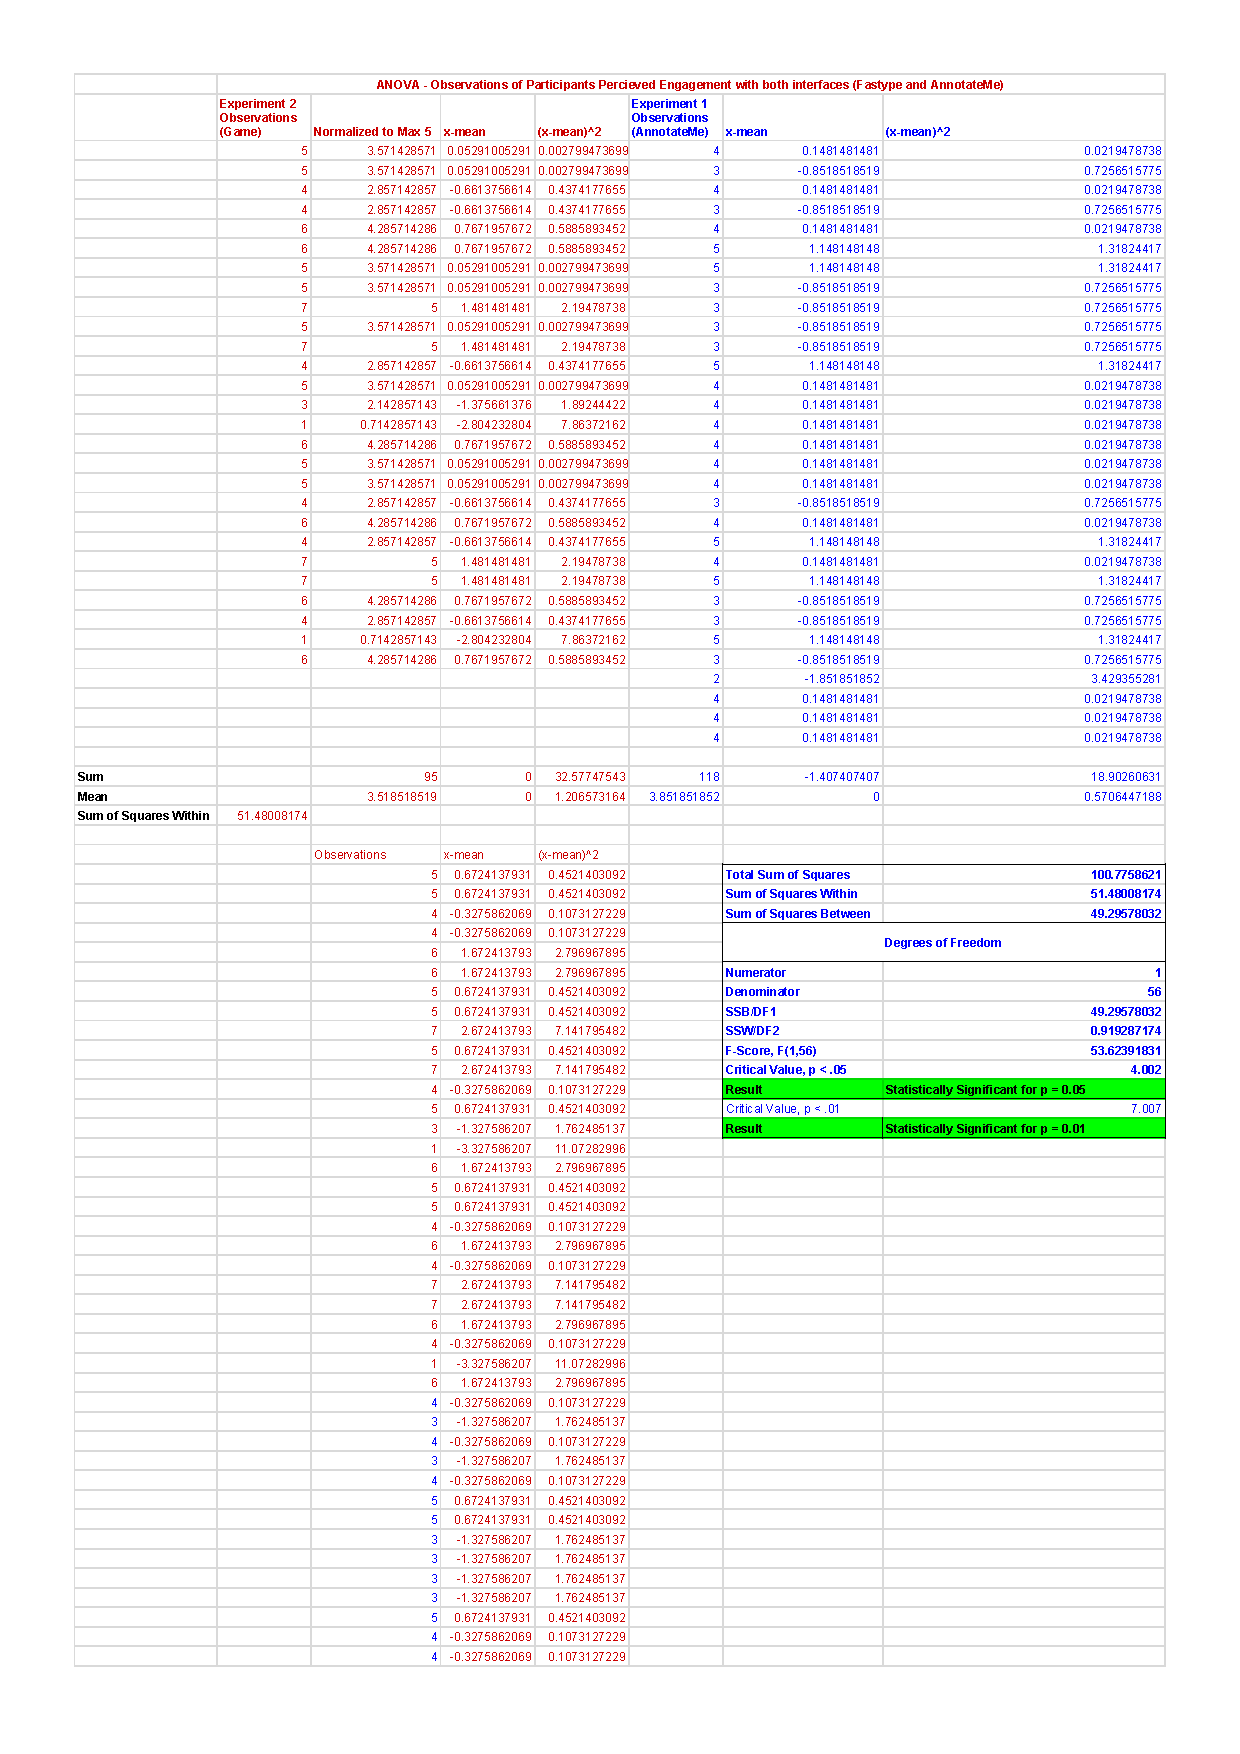
\includepdf[scale=0.7,pages=-]{appendices/participant-engagement.pdf}
